\documentclass{amsart}

\usepackage[T1, T2A]{fontenc}
\usepackage[utf8]{inputenc}
\usepackage{datetime}

\usepackage{amssymb}
\usepackage{amsmath}
\usepackage{amsfonts}

\usepackage{tikz}
\usetikzlibrary{shapes.geometric, arrows}

\tikzstyle{node} = [rectangle, text centered, draw, minimum width=0.5cm, minimum height=0.5cm]
\tikzstyle{arrow} = [thick,->,>=stealth]

\usepackage{fancyhdr}
\usepackage{lipsum}
\usepackage{minted}

\pagestyle{fancy}
\headheight=14pt

\fancyhf{}

\lhead{\largeМатюхин Григорий Васильевич\\НПИбд-01-21, студ. б.: 1032211403}
\rhead{\largeДомашняя работа №1}
\thispagestyle{fancy}

\setcounter{secnumdepth}{0}
\begin{document}

\subsection{1. Точечные пары}

\begin{minted}[mathescape, escapeinside=||]{lisp}
  (('A) 'B) |$\rightarrow$| (('A . NIL) . ('B . NIL))
  (('A . NIL) . ('B . ( 'C . NIL))) |$\rightarrow$| (('A) 'B 'C)
\end{minted}

\subsection{2. Списки}
\begin{minted}[mathescape, escapeinside=||]{lisp}
  ('A ('B) 'C) |$\rightarrow$| ('A . (('B . NIL) . ('C . NIL)))
\end{minted}

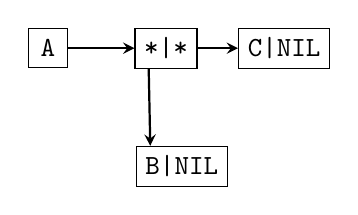
\begin{tikzpicture}[node distance=1.5cm]
  \node (a) [node] {\texttt{A}};
  \node (b) [node, right of=a] {\texttt{*|*}};
  \node (b1) [node, below of=b, xshift=0.2cm] {\texttt{B|NIL}};
  \node (c) [node, right of=b] {\texttt{C|NIL}};

  \draw [arrow] (a) -- (b);
  \draw [arrow] (b) -- (c);

  \draw [arrow] ([xshift=-0.22cm]b.south) -- ([xshift=-0.4cm]b1.north);
\end{tikzpicture}
\\

\begin{minted}[mathescape, escapeinside=||]{lisp}
  ('A 'B ('C)) |$\rightarrow$| ('A . ('B . (('C . NIL) . NIL)))
\end{minted}

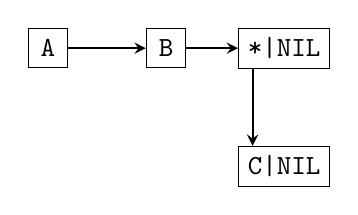
\begin{tikzpicture}[node distance=1.5cm]
  \node (a) [node] {\texttt{A}};
  \node (b) [node, right of=a] {\texttt{B}};
  \node (c) [node, right of=b] {\texttt{*|NIL}};
  \node (c1) [node, below of=c] {\texttt{C|NIL}};

  \draw [arrow] (a) -- (b);
  \draw [arrow] (b) -- (c);

  \draw [arrow] ([xshift=-0.4cm]c.south) -- ([xshift=-0.4cm]c1.north);
\end{tikzpicture}
\\

\begin{minted}[mathescape, escapeinside=||]{lisp}
  (('A) ('B) ('C)) |$\rightarrow$| (('A . NIL) . (('B . NIL) . (('C . NIL) . NIL)))
\end{minted}

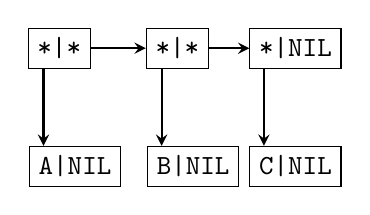
\begin{tikzpicture}[node distance=1.5cm]
  \node (a) [node] {\texttt{*|*}};
  \node (a1) [node, below of=a, xshift=0.2cm] {\texttt{A|NIL}};
  \node (b) [node, right of=a] {\texttt{*|*}};
  \node (b1) [node, below of=b, xshift=0.2cm] {\texttt{B|NIL}};
  \node (c) [node, right of=b] {\texttt{*|NIL}};
  \node (c1) [node, below of=c, xshift=0.0cm] {\texttt{C|NIL}};

  \draw [arrow] (a) -- (b);
  \draw [arrow] (b) -- (c);

  \draw [arrow] ([xshift=-0.2cm]a.south) -- ([xshift=-0.4cm]a1.north);
  \draw [arrow] ([xshift=-0.2cm]b.south) -- ([xshift=-0.4cm]b1.north);
  \draw [arrow] ([xshift=-0.4cm]c.south) -- ([xshift=-0.4cm]c1.north);
\end{tikzpicture}
\\

\begin{minted}[mathescape, escapeinside=||]{lisp}
  ((('AB))) |$\rightarrow$| ((('AB . NIL) . NIL) . NIL)
\end{minted}

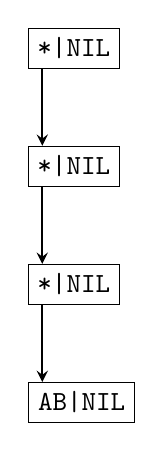
\begin{tikzpicture}[node distance=1.5cm]
  \node (ab) [node] {\texttt{*|NIL}};
  \node (ab1) [node, below of=ab] {\texttt{*|NIL}};
  \node (ab2) [node, below of=ab1] {\texttt{*|NIL}};
  \node (ab3) [node, below of=ab2, xshift=0.1cm] {\texttt{AB|NIL}};

  \draw [arrow] ([xshift=-0.4cm]ab.south) -- ([xshift=-0.4cm]ab1.north);
  \draw [arrow] ([xshift=-0.4cm]ab1.south) -- ([xshift=-0.4cm]ab2.north);
  \draw [arrow] ([xshift=-0.4cm]ab2.south) -- ([xshift=-0.5cm]ab3.north);
\end{tikzpicture}

\end{document}
